\chapter{Snooker - An Overview}
\label{chap:Snooker}

The original objective of this study was to develop a series of enhancements to the synthetic dataset generator SNOOKER. This generator was initially produced by this study's second supervisor Leonardo Silva Ferreira.

SNOOKER was developed to bridge the availability gap for Helpdesk's datasets.

The first step when starting the development phase was to analyse SNOOKER and find out was was running under the hood. In this chapter we will present a general overview of the generator, talking about it's main thecnologies, features and the characteristics of it's syntethicaly genereted datasets.

\section{Technlogies}

SNOOKER was developed using Python and several of its libraries. Python is an interpreted, high-level programming language considered the standard for exploratory interactive and computation-driven scientific research \cite{5725235}. The user-generation interaction was handled by creating a graphical user interface (GUI).

The user interface of the generator was developed using PyQt. PyQt is a combination of Python bindings for cross-platform applications that combine all the strengths of Qt and Python \cite{siahaan2019postgresql}. This enables the development of GUI elements using Python Code. A print of the generator's GUI can be found in Figure \ref{fig:general_gui}.

The user can use the standard parameters in the presented interface or personalize the generation inputs as he wishes, fumbling with several interface options. Upon clicking the Generate button, after a short delay, a synthetical tabular dataset is generated and colocated inside a folder on SNOOKER's file directory.

\begin{figure}[t]
  \begin{center}
    \leavevmode
    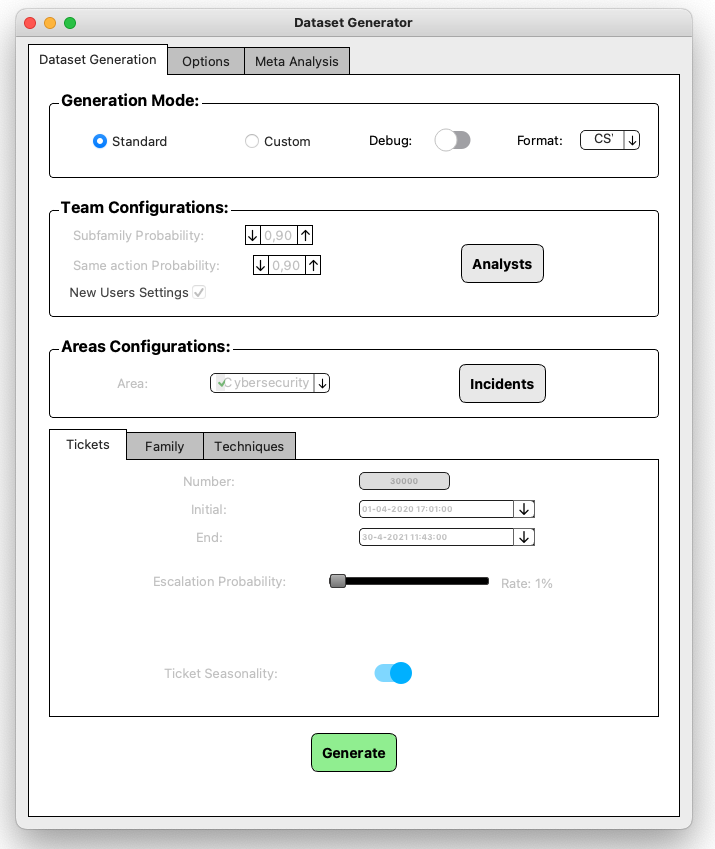
\includegraphics[width=0.6\textwidth]{general_gui.png}
    \caption{SNOOKER's User Interface}
    \label{fig:general_gui}
  \end{center}
\end{figure}

\section{Features}
The primary objective of SNOOKER was to enable synthetic helpdesk dataset generation. This dataset would take into account a series of features. The main features included in the generator are ticket management, team management and area management

Tickets should be able to be customized (quantity, creation time, type, etc.), scheduled, treated (generation of appropriate treatment methods) and replicated if needed. 

The team management module handles both the overhaul statistics of the team (shift management, ticket percentages, etc.) and the singular team member information (general data connected to each member).

Lastly, the area management feature takes care of customizable incidents that might happen in each domain previously described.

It should also be noted that the generator uses as input not only the information provided by the user in the generator's UI but also data from a JSON configuration file.

\section{Synthetic Datasets}
In this section, we will look at the final output from SNOOKER's generation process, explaining the information in each column of the dataset. When looking at the 1st line of the CSV file (the header), we can extract all the columns that will be analysed in this section:
\begin{lstlisting}[breaklines=true]
  ID; Location; Raised (UTC); Allocated; Stages; Fixed; Client; Family; Family Action; Subfamily; Subfamily Action; Subfamily Action Duration; Team; Users in the Shift; Users Next Shift; Users Competent; User actions; User Chosen; Action Chosen; Action Chosen Status; Action Chosen Duration; Action Chosen (With Outlier); Ticket Duration; Escalate; Status; Outlier

\end{lstlisting}

The first column displays the ticket's ID, a unique numerical identifier; in this case, the ID is also the ticket's number. The second column contains the location of the ticket (it's country of origin). Raised (UTC) displays the DateTime the ticket was submitted in UTC format. At the same time, the next column (Allocated) does the same for the time the ticket was allocated to a helpdesk team member. 

Stages register the sub techniques used in the ticket scheduling while also saving data regarding the timestamps of these occurrences. Fixed, like Allotted did before, keeps the DateTime tickets solved. The next metric is simple: the Client column gives information regarding the client the ticket belongs to.

Family, Family Action, Subfamily and Subfamily Action all keep information regarding the nature of the incident that caused that ticket. The Actions metrics save the techniques usually used to solve those problems. Lastly, the Subfamily Action Duration illustrates the time needed to perform the actions presented in the Subfamily Action's column.

Team, Users in the Shift and Users Next Shift give information regarding the team management, the current team, its active members and the members that will become available during the next shift, respectively. Users competent present a list of the most suitable member to perform the task. The User actions column contains data regarding the action that each available user would perform. User Chosen does them present us the team member that will take care of the ticket. Action chosen reflects the action the Chosen user performs, followed by the Action Chosen Status that represents the status of the action chosen. Action Chosen Duration and Action Chosen Duration (With Outlier) display the action's duration and the action's duration if an outlier exists.

The final four columns are Ticket Duration, Escalate, Status and Outlier. The first one depicts the time the ticket has endured without being solved, followed by Escalate, which is responsible for informing the user that the ticket should be passed to the next team. The Status column provides the status of the ticket. Finally, the Outlier notifies us if the ticket should be considered an outlier.


\section{Conclusion}
In this chapter, we performed a simple overview analysis on the current state of SNOOKER. We started by providing a simple explanation of the product where we can see the primary objective it accomplishes. Later we moved on and took a pick at the technologies used to develop the generator. In the Features section we explored the primary models used to create the final syntetic dataset and finaly we showcased the information that derives form the generation process. 